	\subsection{Introduction}


\begin{frame}
  \begin{center}
    {
\includegraphics[height=2cm]{Day1/images/logo_OpenMP.png}}

    \textbf{Lecture based on specifications ver 3.1}

  \end{center}
\end{frame}

\begin{frame}
  \frametitle{Releases history, present and future}
  \begin{itemize}
  \item{October 1997: Fortran version 1.0 }
  \item{Late 1998: C/C++ version 1.0 }
  \item{June 2000: Fortran version 2.0 }
  \item{April 2002: C/C++ version 2.0 }
  \item{June 2005: Combined C/C++ and Fortran version 2.5 }
  \item{May 2008: Combined C/C++ and Fortran version  3.0}
  \item{\textbf{July 2011: Combined C/C++ and Fortran version  3.1}}
  \item{July 2013: Combined C/C++ and Fortran version 4.0 }
  \item{November 2015: Combined C/C++ and Fortran version 4.5 }
  \end{itemize}
\end{frame}

% \subsubsection{threading concepts, terminology (OpenMP, tasking, data, implementation)}

\begin{frame}
  \frametitle{Terminology}
  \begin{itemize}
  \item{\textbf{thread :} an execution entity with a stack and a static memory (\textit{threadprivate memory})}
  \item{\textbf{OpenMP thread :} a \textit{thread} managed by the OpenMP runtime}
  \item{\textbf{thread-safe routine :} a routine that can be executed concurrently}
  \item{\textbf{processor :} an HW unit on which one or more \textit{OpenMP thread} can execute}
%  \item{\textbf{device :} an implementation defined logical execution engine}
  \end{itemize}
\end{frame}

\subsubsection{Models}

\begin{frame}
  \frametitle{Execution and memory models}
  \begin{itemize}
  \item{Execution model : fork-join}
  \item{One heavy thread (process) per program (initial thread)}
  \item{leightweigt threads for parallel regions. threads are assigned to cores by the OS}
  \item{No implicit synchronization (except at the beginning and at the end of a parallel region)}
  \item{Shared Memory with shared variables}
  \item{Private Memory per thread with threadprivate variables}
  \end{itemize}
\end{frame}

\begin{frame}
  \frametitle{Memory model (simplified)}
  \begin{center}
    {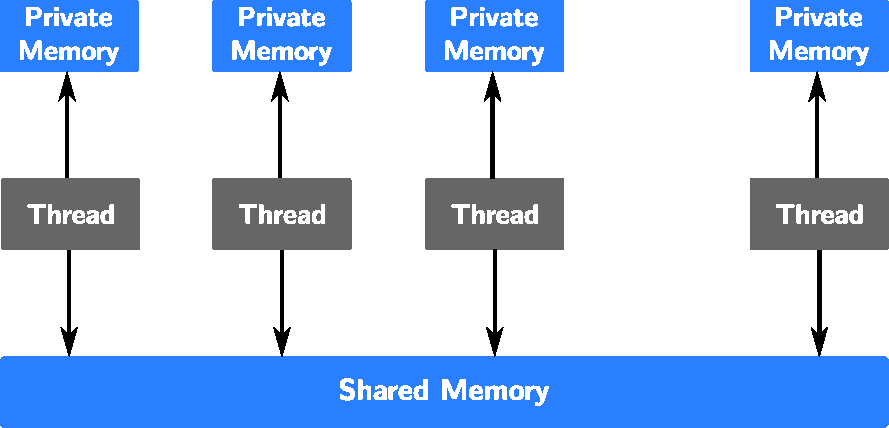
\includegraphics[width=\textwidth]{Day1/images/memory-model-simplified.pdf}}
  \end{center}
\end{frame}

\begin{frame}
  \frametitle{Execution model (simplified)}
  \begin{center}
    {% Slide 72
\begin{tikzpicture}[yscale = 0.7, xscale = 0.9]

\draw[very thick, ->] (0,8.5) node[above right] {Master thread} -- (0,-1);

\pgfmathsetmacro{\forkheight}{7}

\foreach \x in {1, 2, ..., 5} {
	\draw[blue2, ->, thick] (0,{\forkheight + 0.5})
		to[out = -90, in = 180] (0.5, \forkheight)
		-- ({\x - 0.5}, \forkheight)
		to[out=0, in = 90] (\x, {\forkheight-0.5}) -- (\x, {\forkheight - 2});

	\draw[blue2, thin] (\x, {\forkheight - 2})
		to[out = -90, in = 0] ({\x - 0.5}, {\forkheight - 2.25})
		-- (0.5, {\forkheight - 2.25})
		to[out = 180, in = 90] (0, {\forkheight - 2.5});
}

\node[point, label={left:Fork}] at (0, {\forkheight + 0.5}) {};
\node[point, label={left:Join}] at (0, {\forkheight - 2.5}) {};
\node[blue2, anchor = south, yshift = 0.1cm] at (4, \forkheight) {Worker threads};

\pgfmathsetmacro{\forkheight}{2.5}

\foreach \x in {1, 2, 3} {
	\draw[blue2, ->, thick] (0,{\forkheight + 0.5})
		to[out = -90, in = 180] (0.5, \forkheight)
		-- ({\x - 0.5}, \forkheight)
		to[out=0, in = 90] (\x, {\forkheight-0.5}) -- (\x, {\forkheight - 2});

	\draw[blue2, thin] (\x, {\forkheight - 2})
		to[out = -90, in = 0] ({\x - 0.5}, {\forkheight - 2.25})
		-- (0.5, {\forkheight - 2.25})
		to[out = 180, in = 90] (0, {\forkheight - 2.5});
}

\node[blue2, anchor = south, yshift = 0.1cm] at (2, \forkheight) {Worker threads};

\node[point, label={left:Fork}] at (0, {\forkheight + 0.5}) {};
\node[point, label={left:Join}] at (0, {\forkheight - 2.5}) {};

\end{tikzpicture}
}
  \end{center}
\end{frame}

\subsubsection{Remarks}

\begin{frame}
  \frametitle{OpenMP and MPI/pthreads	}
  \begin{itemize}
  \item{\textbf{OpenMP} $\neq$ OpenMPI}
  \item{All what you can do with OpenMP can be done with MPI and/or pthreads}
    % \item{Memory issue}
  \item{easier \textbf{BUT} data coherence/consistency}
    % \item{In fact: \textbf{no} easy parallel paradigm exists}
  \end{itemize}
\end{frame}

\subsection{Directives}

\subsubsection{format \& conditional compilation}

\begin{frame}[containsverbatim]
  \frametitle{Syntax in C}
  % \begin{itemize}
  % \item{OpenMP directives are written as pragmas: \texttt{\#pragma omp}}
  % \item{Use the conditional compilation flag \texttt{\#if defined \_OPENMP} for the preprocessor}
  % \end{itemize}

  \begin{block}{}
    OpenMP directives are written as pragmas: \texttt{\#pragma omp}
  \end{block}

  \begin{block}{}
    Use the conditional compilation flag \texttt{\#if defined \_OPENMP} for the preprocessor
  \end{block}

  Compilation using the GNU gcc or Intel compiler:
\begin{verbatim}
gcc -fopenmp ex1.c -o ex1
\end{verbatim}
\end{frame}


\begin{frame}[containsverbatim]
  \frametitle{Hello World in C}

  \begin{lstlisting}[language=C++,frame=lines]
#include <stdio.h>
#include <omp.h>
int main(int argc, char *argv[]) {
   int myrank=0;
   int mysize=1;
#if defined (_OPENMP)
#pragma omp parallel default(shared) private(myrank, mysize)
{
   mysize = omp_get_num_threads();
   myrank = omp_get_thread_num();
#endif
   printf("Hello from thread %d out of %d\n", myrank, mysize);
#if defined (_OPENMP)
}
#endif
   return 0;
}
\end{lstlisting}
% (Source file: \texttt{ex1.c})
\end{frame}

\begin{frame}[containsverbatim]
  \frametitle{Syntax in Fortran 90}
  % \begin{itemize}
  % \item{OpenMP directives are written as comments: \texttt{!\$omp omp}}
  % \item{Sentinels \texttt{!\$} are authorized for conditional compilation  (preprocessor) }
  % \end{itemize}

  \begin{block}{}
    OpenMP directives are written as comments: \texttt{!\$omp omp}
  \end{block}
  \begin{block}{}
    Sentinels \texttt{!\$} are authorized for conditional compilation  (preprocessor)
  \end{block}


  Compilation using the GNU gfortran or Intel ifort compiler:
\begin{verbatim}
gfortran -fopenmp ex1.f90 -o ex1
\end{verbatim}
\end{frame}



\begin{frame}[containsverbatim]
  \frametitle{Hello World in Fortran 90}

  \begin{lstlisting}[language=Fortran,frame=lines]
program ex1
   implicit none
   integer :: myrank, mysize
!$ integer, external :: omp_get_num_threads, omp_get_thread_num
   myrank=0
   mysize=1
!$omp   parallel default(shared) private(myrank, mysize)
!$      mysize = omp_get_num_threads()
!$      myrank = omp_get_thread_num()
   print *, "Hello from thread",myrank,"out of",mysize
!$omp   end parallel
end program ex1
\end{lstlisting}
% $ This comment is just for the colors in emacs...
\end{frame}

\begin{frame}[containsverbatim]
  \frametitle{Number of concurrent threads}

  The number of threads is specified in a hardcoded way ($omp\_set\_num\_threads()$) or via an environment variable.
  \\~\\

  BASH-like shells :

\begin{verbatim}
export OMP_NUM_THREADS=4
\end{verbatim}

  CSH-like shells :

\begin{verbatim}
setenv OMP_NUM_THREADS 4
\end{verbatim}
\end{frame}


\begin{frame}[containsverbatim]
  \frametitle{Components of OpenMP}
  \begin{itemize}
  \item{Compiler directives (written as comments) that allow work sharing, synchronization and data scoping}
  \item{A runtime library (libomp.so) that contains informal, data access and synchronization directives}
  \item{Environment variables}
  \end{itemize}
\end{frame}


\subsubsection{The \texttt{parallel} construct}


\begin{frame}[containsverbatim]
  \frametitle{The \texttt{parallel} construct}

  \begin{exampleblock}{Syntax}
    This is the mother of all constructs in OpenMP. It starts a parallel execution.
    \begin{lstlisting}[language=C,frame=lines]
#pragma omp parallel [clause[[,] clause]...]
{
   structured-block
}
\end{lstlisting}
    where \textit{clause} is one of the following:
    \begin{itemize}
    \item \textbf{\texttt{if}} or \textbf{\texttt{num\_threads}} : conditional clause
    \item \textbf{\texttt{default(private | firstprivate | shared | none)}} : default data scoping
    \item \textbf{\texttt{private(\textit{list})}}, \textbf{\texttt{firstprivate(\textit{list})}}, \textbf{\texttt{shared(\textit{list})}} or \textbf{\texttt{copyin(\textit{list})}} : data scoping
    \item \textbf{\texttt{reduction(\textit{\{ operator | intrinsic\_procedure\_name \} : list})}}
    \end{itemize}
  \end{exampleblock}
\end{frame}


\begin{frame}[fragile]
  \frametitle{Example : the \texttt{if} conditional clause }

  \begin{block}{The \texttt{if} clause}
    A \texttt{if} test specifies if a parallel region must be executed in parallel or not:

\begin{verbatim}
if (n<2) then
   execute test(n) serial
else
   execute test(n) in parallel
endif
\end{verbatim}

  \end{block}

  \begin{lstlisting}[language=C,frame=lines]
#pragma omp parallel if (n>2)
   test(n);
\end{lstlisting}
\end{frame}

\begin{frame}[containsverbatim]
  \frametitle{The \texttt{if} clause [output]}

\begin{verbatim}
vkeller@mathicsepc13:~/OpenMP/exercises/C$ ./ex3
 var =       1  : Code is executed by only one thread
 Parallelized with           2 threads :            2
 Parallelized with           3 threads :            3
 Parallelized with           4 threads :            4
\end{verbatim}

\end{frame}


\begin{frame}[containsverbatim]
  \frametitle{Data scoping}
  What is data scoping ?
  \begin{itemize}
  \item{most common source of errors}
  \item{determine which variables are {\bf private} to a thread, which are {\bf shared} among all the threads}
  \item{In case of a private variable, what is its value when entering the
      parallel region {\bf firstprivate}, what is its value when leaving the
      parallel region {\bf lastprivate}}
  \item The default scope (if none are specified) is \textbf{shared}
  \item{most difficult part of OpenMP}
  \end{itemize}
\end{frame}


\begin{frame}[fragile]
  \frametitle{The data sharing-attributes \texttt{shared} and \texttt{private}}
  \begin{exampleblock}{Syntax}
These attributes determines the scope (visibility) of a single or list of variables
\begin{lstlisting}[language=C,frame=lines]
shared(list1) private(list2)
\end{lstlisting}

\begin{itemize}
\item{The \verb+private+ attribute : the data is private to each thread and non-initiatilized. Each thread has its own copy. Example : \verb+#pragma omp parallel private(i)+}
\item{The \verb+shared+ attribute : the data is shared among all the threads. It is accessible (and non-protected) by all the threads simultaneously. Example : \verb+#pragma omp parallel shared(array)+}
\end{itemize}

\end{exampleblock}

\end{frame}



\begin{frame}[containsverbatim]
\frametitle{The data sharing-attributes \texttt{firstprivate} and \texttt{lastprivate}}
\begin{exampleblock}{Syntax}
These clauses determines the attributes of the variables within a parallel region:
\begin{lstlisting}[language=C,frame=lines]
firstprivate(list1) lastprivate(list2)
\end{lstlisting}
\begin{itemize}
\item{The \texttt{firstprivate} like {\tt private} but initialized to the value before the parallel region}
\item{The \texttt{lastprivate}  like {\tt private} but the value is updated after the parallel region}
\end{itemize}
\end{exampleblock}
%\begin{alertblock}{}
%\textbf{Fortran only !}
%\end{alertblock}
\end{frame}




\subsubsection[Worksharing constructs]{worksharing constructs ("subsubsections", "single", "workshare")}



\begin{frame}[containsverbatim]
\frametitle{Worksharing constructs}

\begin{block}{}
Worksharing constructs are possible in three ``flavours'' :
\begin{itemize}
\item{\textbf{\texttt{sections}} construct}
\item{\textbf{\texttt{single}} construct}
%\item{\textbf{\texttt{master}} construct}
\item{\textbf{\texttt{workshare}} construct (only in Fortran)}
\end{itemize}
\end{block}

\end{frame}

\begin{frame}[containsverbatim]
\frametitle{The \texttt{sections} construct}
\begin{exampleblock}{Syntax}

\begin{lstlisting}[language=C,frame=lines]
#pragma omp [parallel] sections [clause]
{
   #pragma omp section
   {
      code_block
   }
}\end{lstlisting}
where \textit{clause} is one of the following:
\begin{itemize}
\item{\textbf{\texttt{private(\textit{list})}}, \textbf{\texttt{firstprivate(\textit{list})}}, \textbf{\texttt{lastprivate(\textit{list})}} : data scoping}
\item{\textbf{\texttt{reduction(\textit{\{ operator | intrinsic\_procedure\_name \} : list})}} : data scoping}
\item{Each \textbf{\texttt{section}} within a \textbf{\texttt{sections}} construct is assigned to one and only one thread}
\end{itemize}
\end{exampleblock}


\end{frame}


\begin{frame}[containsverbatim]
\frametitle{A \texttt{sections} construct example (Exercise)}


\begin{block}{Example}
\begin{verbatim}
#pragma omp parallel
#pragma omp sections
{
  #pragma omp section
       do something from a thread
  #pragma omp section
       do something from another thread
  #pragma omp section
       do something from another thread
}
\end{verbatim}
\end{block}

\end{frame}


\begin{frame}[containsverbatim]
\frametitle{The \texttt{single} construct}

\begin{exampleblock}{Syntax}
\begin{lstlisting}[language=C,frame=lines]
#pragma omp single [clause[[,] clause] ...]
{
   structured-block
}
\end{lstlisting}
where \textit{clause} is one of the following:
\begin{itemize}
\item{\textbf{\texttt{private(\textit{list})}}, \textbf{\texttt{firstprivate(\textit{list})}}}
\end{itemize}
\end{exampleblock}

\begin{block}{}
Only one thread (usualy the first entering thread) executes the \textbf{\texttt{single}} region. The others wait for completion, except if the \textbf{\texttt{nowait}} clause has been activated
\end{block}

\end{frame}


\begin{frame}[containsverbatim]
\frametitle{The \texttt{master} construct}

\begin{itemize}
        \item{Only the master thread execute the section. It can be used in any OpenMP construct}
\end{itemize}

\begin{lstlisting}[language=C,frame=lines]
#pragma omp parallel default(shared)
{
...
   #pragma omp master
   {
      printf("I am the master\n");
   }
...
}
\end{lstlisting}

\end{frame}


\begin{frame}[containsverbatim]
\frametitle{The \texttt{workshare} construct (\textbf{only Fortran})}
\begin{exampleblock}{Syntax}
\begin{lstlisting}[language=Fortran,frame=lines]
!$omp workshare
   structured-block
!$omp end workshare [nowait]
\end{lstlisting}
The enclosed structured block must consist of only the following:
\begin{itemize}
\item{array and scalar assignements}
\item{\textbf{\texttt{FORALL}} statements and constructs}
\item{\textbf{\texttt{WHERE}} statements and constructs}
\item{\textbf{\texttt{atomic}} constructs}
\item{\textbf{\texttt{critical}} constructs}
\item{\textbf{\texttt{parallel}} constructs}
\end{itemize}
\end{exampleblock}
\end{frame}



\begin{frame}[containsverbatim]
\frametitle{A \texttt{workshare} construct example}
\begin{lstlisting}[language=Fortran,frame=lines]
!$omp parallel shared(A,B) private(i,j)
!$omp workshare
forall (i=1:N, j=1:N, A(i,j).NE.0.)
   A(i,j) = 3*A(i,j)/.23 + 6.
   B(i,j) = A(i,j) ** 2
end forall
!$omp end workshare
!$omp end parallel
\end{lstlisting}

\end{frame}


\subsubsection[Loops]{loops}

\begin{frame}[containsverbatim]
\frametitle{The \texttt{for} directive}

\begin{block}{}
Parallelization of the following loop
\end{block}

\begin{exampleblock}{Syntax}
\begin{lstlisting}[language=C,frame=lines]
#pragma omp for [clause[[,] clause] ... ]
{
   for-loop
}
\end{lstlisting}
where \textit{clause} is one of the following:
\begin{itemize}
\item{\textbf{\texttt{schedule(\textit{kind[, chunk\_size]})}}}
\item{\textbf{\texttt{collapse(\textit{n})}}}
\item{\textbf{\texttt{ordered}}}
\item{\textbf{\texttt{private(\textit{list})}}, \textbf{\texttt{firstprivate(\textit{list})}}, \textbf{\texttt{lastprivate(\textit{list})}},\texttt{reduction()} }
\end{itemize}
\end{exampleblock}
\end{frame}


\begin{frame}[containsverbatim]
\frametitle{The \texttt{reduction(...)} clause (Exercise)}
\begin{block}{How to deal with}
\vspace{-.5cm}
\begin{verbatim}
vec = (int*) malloc (size_vec*sizeof(int));
global_sum = 0;
for (i=0;i<size_vec;i++){
   global_sum += vec[i];
}
\end{verbatim}
\end{block}

\vspace{-.5cm}
\begin{block}{A solution with the \texttt{reduction(...)} clause}
\vspace{-.5cm}

\begin{verbatim}
vec = (int*) malloc (size_vec*sizeof(int));
global_sum = 0;
#pragma omp parallel for reduction(+:global_sum)
   for (i=0;i<size_vec;i++){
      global_sum += vec[i];
   }
\end{verbatim}
But other solutions exist !
\end{block}
\end{frame}


\begin{frame}[containsverbatim]
\frametitle{The \texttt{schedule} clause}

\begin{block}{}
Load-balancing
\end{block}

\begin{center}
\begin{tabular}{|l|l|}
\hline
  \textbf{clause} & \textbf{behavior}  \\
\hline
\hline
\textit{schedule(static [, chunk\_size])} &
iterations divided in chunks sized \\
& \textit{chunk\_size} assigned to threads in \\
& a round-robin fashion.  \\
& If \textit{chunk\_size} not specified \\
& system decides. \\
\hline

\textit{schedule(dynamic [, chunk\_size])} &
iterations divided in chunks sized \\
& \textit{chunk\_size} assigned to threads \\
& when they request them until no \\
& chunk remains to be distributed. \\
& If \textit{chunk\_size} not specified \\
& default is 1. \\

\hline
\end{tabular}
\end{center}

\end{frame}


\begin{frame}[containsverbatim]
\frametitle{The \texttt{schedule} clause}

\begin{center}
\begin{tabular}{|l|l|}
\hline
  \textbf{clause} & \textbf{behavior}  \\
\hline
\hline
\textit{schedule(guided [, chunk\_size])}  &
iterations divided in chunks sized \\
& \textit{chunk\_size} assigned to threads \\
& when they request them. Size of  \\
& chunks is proportional to the  \\
& remaining unassigned chunks. \\
%& If \textit{chunk\_size} not specified \\
%& default is 1. \\
& By default the chunk size is approx \\
& loop$\_$count/number$\_$of$\_$threads. \\

%By default the chunk size is approximately 


\hline
\textit{schedule(auto)}  &
The decisions is delegated to the \\
 & compiler and/or the runtime system \\

\hline
\textit{schedule(runtime)}  &
The decisions is delegated to the \\
 & runtime system \\


\hline
\end{tabular}
\end{center}

\end{frame}


\begin{frame}
\frametitle{The \texttt{schedule} clause}
\begin{center}
{% Slide 97
\begin{tikzpicture}[scale=0.8]

\node (Start) at (0, 4) {Start};
\node[decision] (Schedule) at (0, 2) {\texttt{schedule} \\ clause present?};
\node[anchor = west] (DefSched) at (4, 2) {Use \textit{def-sched-var} schedule kind};
\node[decision, inner sep = 2pt] (Runtime) at (0, -1.5) {schedule kind \\ value is \texttt{runtime}?};
\node[anchor = west, align = left] (SchedKind) at (4, -1.5) {Use schedule kind specified\\ in \texttt{schedule} clause};
\node[anchor = west, align = left] (RunSched) at (4, -4) {Use \textit{run-sched-var} schedule kind};

\draw[->] (Start) -- (Schedule);
\draw[->] (Schedule) -- node[near start, above] {No} (DefSched);
\draw[->] (Schedule) -- node[midway, right] {Yes} (Runtime);
\draw[->] (Runtime) |- node[pos = 0.83, above] {Yes} (RunSched);
\draw[->] (Runtime) -- node[near start, above] {No} (SchedKind);
\end{tikzpicture}
}
\end{center}
\end{frame}


\begin{frame}[containsverbatim]
\frametitle{A parallel \texttt{for} example}


\begin{block}{How to...}
... parallelize the dense matrix multiplication $C = A B$ (triple for loop $C_{ij} = C_{ij} + A_{ik} B_{kj}$). What happens using different \texttt{schedule} clauses ?)
\end{block}

\end{frame}


\begin{frame}[containsverbatim]
\frametitle{A parallel \texttt{for} example}
\begin{lstlisting}[language=C,frame=lines]
   #pragma omp parallel shared(A,B,C) private(i,j,k,myrank)
   {
      myrank=omp_get_thread_num();
      mysize=omp_get_num_threads();
      chunk=(N/mysize);
      #pragma omp for schedule(static, chunk)
      for (i=0;i<N;i++){
         for (j=0;j<N;j++){
            for (k=0;k<N;k++){
               C[i][j]=C[i][j] + A[i][k]*B[k][j];
            }
         }
      }
   }
\end{lstlisting}
%Loop order is important !
\end{frame}

\begin{frame}[containsverbatim]
\frametitle{A parallel \texttt{for} example}

\begin{verbatim}
vkeller@mathicsepc13:~$ export OMP_NUM_THREADS=1
vkeller@mathicsepc13:~$ ./a.out
 [DGEMM] Compute time [s]   : 0.33388209342956
 [DGEMM] Performance  [GF/s]: 0.59901385529736
 [DGEMM] Verification       : 2000000000.00000
vkeller@mathicsepc13:~$ export OMP_NUM_THREADS=2
vkeller@mathicsepc13:~$ ./a.out
 [DGEMM] Compute time [s]   : 0.18277192115783
 [DGEMM] Performance  [GF/s]: 1.09425998661625
 [DGEMM] Verification       : 2000000000.00000
vkeller@mathicsepc13:~$ export OMP_NUM_THREADS=4
vkeller@mathicsepc13:~$ ./a.out
 [DGEMM] Compute time [s]   : 9.17780399322509E-002
 [DGEMM] Performance  [GF/s]: 2.17917053085506
 [DGEMM] Verification       : 2000000000.00000
\end{verbatim}

\end{frame}




\begin{frame}
\frametitle{The \texttt{collapse} clause}

\begin{block}{Intel view}
Use the collapse clause to increase the total number of iterations that will be partitioned across the available number of OMP threads by reducing the granularity of work to be done by each thread.

You can improve performance by avoiding use of the collapsed-loop indices (if possible) inside the collapse loop-nest (since the compiler has to recreate them from the collapsed loop-indices using divide/mod operations AND the uses are complicated enough that they don't get dead-code-eliminated as part of compiler optimizations)
\end{block}

\end{frame}

\begin{frame}[containsverbatim]
\frametitle{A \texttt{collapse} directive example}

\begin{lstlisting}[language=C,frame=lines]
#pragma omp parallel for collapse(2) shared(A) private(k,l)
   for (k=0;k<kmax;k++) {
      for (l=0;l<lmax;l++){
         do_some_work(&A,k,l,N);
      }
   }
\end{lstlisting}
where \texttt{do\_some\_work(A,k,l,N)} looks like:
\begin{lstlisting}[language=C,frame=lines]
   for(i=0;i<N;i++) {
      for (j=0;j<N;j++) {
         A[i][j] = A[i][j]*s+A[i][j]*t
      }
   }
\end{lstlisting}
\end{frame}

\begin{frame}[containsverbatim]
\frametitle{A \texttt{collapse} directive example [output]}
\begin{block}{}
Here we compare the collapsed result with the standard parallel loop (on \texttt{k})
\end{block}

%\begin{table}
%\begin{center}
\begin{tabular}{|l|l|l|l|l|l|}
\hline
 \textbf{OMP\_NUM\_THREADS} & \textbf{1} & \textbf{2} & \textbf{4} & \textbf{8} & \textbf{16}\\
\hline
\hline
standard // loop &2.17 &1.69 &1.69 &1.44 &1.22 \\
\hline
collapsed(2) // loop &2.13 &1.60 &1.02 &0.83 &0.70 \\
\hline
\end{tabular}
%\end{center}
%\caption{\texttt{N=20000}, time is in seconds}
%\end{table}

\texttt{N=20000}, time is in seconds

\begin{block}{Remark}
It is mandatory that the \textit{\texttt{n-}}collapsed loops are perfectly nested and with a rectangular shape (nothing like \texttt{do i=1,N ... do j=1,f(i)}) and that their upper limits are ``small''.
\end{block}



\end{frame}




\subsubsection{tasking constucts ("task", "taskyield")}

\begin{frame}[containsverbatim]
\frametitle{The \texttt{task} directive}
\begin{center}
    {% Slide 104
\begin{tikzpicture}[scale = 0.9]
\begin{scope}

\node[anchor = east] at (0,0) {Master thread};
\draw (0,0) -- (9.6, 0);
\draw[line width = 3pt, blue6, opacity = 0.4] (0,0) -- (9.6, 0);

\node[anchor = south] at (2.2, 0.6) {Task 1};
\draw[thick, fill = white] (1, -0.6) rectangle (3.4, 0.6);
\draw (1, -0.4) -- (3.4, -0.4);
\draw (1, 0.4) -- (3.4, 0.4);
\draw (1.8, 0.4) -- (1.8, -0.4);
\draw (2.6, 0.4) -- (2.6, -0.4);

\node at (1.4, 0) {A};
\node at (2.2, 0) {B};
\node at (3, 0) {C};

\node[anchor = south] at (5.2, 0.6) {Task 2};
\draw[thick, fill = white] (4, -0.6) rectangle (6.4, 0.6);
\draw (4, -0.4) -- (6.4, -0.4);
\draw (4, 0.4) -- (6.4, 0.4);
\draw (4.6, 0.4) -- (4.6, -0.4);
\draw (5.0, 0.4) -- (5.0, -0.4);
\draw (5.9, 0.4) -- (5.9, -0.4);

\node at (4.3, 0) {A};
\node at (4.8, 0) {B};
\node at (5.45, 0) {C};
\node at (6.15, 0) {D};

\node[anchor = south] at (8.2, 0.6) {Task 3};
\draw[thick, fill = white] (7, -0.6) rectangle (9.4, 0.6);
\draw (7, -0.4) -- (9.4, -0.4);
\draw (7, 0.4) -- (9.4, 0.4);

\draw (8.2, -0.4) -- (8.2, 0.4);
\node at (7.6, 0) {A};
\node at (8.8, 0) {B};
\end{scope}

\begin{scope}[yshift = -3cm]

\node[anchor = east] at (0,0) {Master thread};
\draw (0,0) -- (9.6, 0);

\node[anchor = south] at (1.7, 1.5) {\scriptsize Parallel Task 1};
\draw[thick, fill = white] (1, -1.5) rectangle (2.4, 1.5);

\node[anchor = south] at (3.9, 1.5) {\scriptsize Parallel Task 2};
\draw[thick, fill = white] (3.2, -1.5) rectangle (4.6, 1.5);

\node[anchor = south] at (6.3, 1.5) {\scriptsize Parallel Task 3};
\draw[thick, fill = white] (5.4, -1.5) rectangle (7.2, 1.5);

\node[draw, rectangle, minimum width = 0.8cm, minimum height = 0.8cm] (A1) at (1.7, 0.9) {A};
\node[draw, rectangle, minimum width = 0.8cm, minimum height = 0.8cm] (B1) at (1.7, 0.0) {B};
\node[draw, rectangle, minimum width = 0.8cm, minimum height = 0.8cm] (C1) at (1.7, -0.9) {C};
\node[draw, rectangle, minimum width = 0.6cm, minimum height = 0.5cm] (A2) at (3.75, 1) {A};
\node[draw, rectangle, minimum width = 0.4cm, minimum height = 0.5cm] (B2) at (3.7, 0.35) {B};
\node[draw, rectangle, minimum width = 0.9cm, minimum height = 0.5cm] (C2) at (3.9, -0.35) {C};
\node[draw, rectangle, minimum width = 0.5cm, minimum height = 0.5cm] (D2) at (3.725, -1) {D};
\node[draw, rectangle, minimum width = 1.2cm, minimum height = 0.8cm] (A3) at (6.3, 0.75) {A};
\node[draw, rectangle, minimum width = 1.2cm, minimum height = 0.8cm] (B3) at (6.3, -0.75) {B};

\draw[line width = 3pt, blue6, opacity = 0.4] (0,0) -- (1, 0) -- (A1.west) (A1.east) -- (2.4,0) -- (3.2, 0) -- (A2.west) (A2.east) -- (4.4, 1) -- (4.6, 0) -- (5.4, 0) -- (A3.west) (A3.east) -- (7.2, 0) -- (9.6, 0);

\draw[dashed] (1, 0) -- (A1.west) (A1.east) -- (2.4, 0);
\draw[dashed] (1, 0) -- (B1.west) (B1.east) -- (2.4, 0);
\draw[dashed] (1, 0) -- (C1.west) (C1.east) -- (2.4, 0);

\draw[dashed] (3.2, 0) -- (A2.west) (A2.east) -- (4.4, 1) -- (4.6, 0);
\draw[dashed] (3.2, 0) -- (B2.west) (B2.east) -- (4.4, 0.35) -- (4.6, 0);
\draw[dashed] (3.2, 0) -- (C2.west) (C2.east) -- (4.4, -0.35) -- (4.6, 0);
\draw[dashed] (3.2, 0) -- (D2.west) (D2.east) -- (4.4, -1) -- (4.6, 0);

\draw[dashed] (5.4, 0) -- (A3.west) (A3.east) -- (7.2, 0);
\draw[dashed] (5.4, 0) -- (B3.west) (B3.east) -- (7.2, 0);

\end{scope}

\end{tikzpicture}

}
\end{center}
Source : wikipedia.org
\end{frame}


\begin{frame}[containsverbatim]
\frametitle{The \texttt{task} directive}

\begin{exampleblock}{What is an OpenMP task ?}
\begin{itemize}
\item{Offers a solution to parallelize irregular problems (unbounded loops, recursives, master/slave schemes, etc..)}
\item{OpenMP tasks are composed of
        \begin{itemize}
        \item{\textbf{code} : what will be executed}
        \item{\textbf{data} : initialized at task creation time }
        \item{\textbf{ICV's} : Internal Control Variables }
        \end{itemize}
}
\end{itemize}
\end{exampleblock}

\begin{exampleblock}{Synchronization}
\begin{itemize}
\item{All tasks created by a thread of a team are garanteed to be completed at
    thread exit (end of block)}
\item{Within a task group, it is possible to synchronize through \texttt{\#pragma
      omp taskwait}}
\end{itemize}
\end{exampleblock}
\end{frame}


\begin{frame}[containsverbatim]
\frametitle{The \texttt{task} directive}

\begin{exampleblock}{Syntax}
\begin{lstlisting}[language=C,frame=lines]
#pragma omp task [clause[[,] clause] ...] 
{
  structured-block
}
\end{lstlisting}
where \textit{clause} is one of the following:
\begin{itemize}
\item{\textbf{\texttt{if(\textit{scalar-logical-expression})}}}
\item{\textbf{\texttt{final(\textit{scalar-logical-expression})}}}
\item{\textbf{\texttt{untied}}}
\item{\textbf{\texttt{default (private | firstprivate | shared | none)}}}
\item{\textbf{\texttt{mergeable}}}
\item{\textbf{\texttt{private(\textit{list})}}, \textbf{\texttt{firstprivate(\textit{list})}}, \textbf{\texttt{shared(\textit{list})}}}
\end{itemize}
\end{exampleblock}
\end{frame}



\begin{frame}[containsverbatim]
\frametitle{The \texttt{task} directive}

\begin{exampleblock}{Execution model}
\begin{itemize}
\item{A task \texttt{t} is executed by the thread \texttt{T} of the team that generated it. Immediately or not (depends on the implementation)}
\item{A thread \texttt{T} can suspend/resume/restart a task \texttt{t}}
\item{Tasks are \textbf{tied} by default:
        \begin{itemize}
        \item{tied tasks are executed by the same thread}
        \item{tied tasks have scheduling restrictions (deterministic creation, synchronization, destruction)}
        \end{itemize}
}
\item{It is possible to untie tasks with the directive \texttt{untied}}
\end{itemize}
\end{exampleblock}


\end{frame}


\begin{frame}[containsverbatim]
\frametitle{A \texttt{task} directive (stupid) example}

You probably know this popular example to compute the \texttt{n} first Fibonacci numbers (Fib = [1,1,2,3,5,8,13,21,34,..]):

\begin{columns}
%\begin{column}[l]{7cm}
\begin{column}{7cm}

\begin{lstlisting}[language=C,frame=lines]
int fibonacci(int n){
   int x,y;
   if (n < 2) {
      return n;
   } else {
      x = fibonacci(n-1);
      y = fibonacci(n-2);
      return (x+y);
   }
}
\end{lstlisting}

\end{column}
\begin{column}[c]{3cm}
{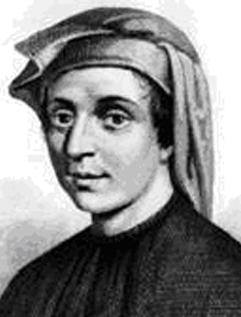
\includegraphics[height=4cm]{Day1/images/Fibonacci.jpg}}
\end{column}
\end{columns}

\end{frame}

\begin{frame}[containsverbatim]
\frametitle{A \texttt{task} directive (stupid) example (Exercise)}

\begin{block}{Idea}
The idea is using the {\tt \#pragma omp tasks} construct by spawning a new task whenever the recursive function is called.
\begin{verbatim}
   ! start the following call in a task
      x=fibonacci(n-1)
   ! start the following call in a task
      y=fibonacci(n-2)
   ! a synchronization must be done here !
      fibonacci = (x+y)
\end{verbatim}

\end{block}

\begin{alertblock}{Warning: number of tasks and number of physical cores}
Pay attention to the number of tasks with respect to the number of cores you have on the node (here 48).
\end{alertblock}
\end{frame}



\begin{frame}[containsverbatim]
\frametitle{A \texttt{task} directive (stupid) example}
\begin{lstlisting}[language=C,frame=lines]
int fibonacci(int n){
   int x,y;
   if (n < 2) {
      return n;
   } else {
#pragma omp task shared(x)
      x = fibonacci(n-1);
#pragma omp task shared(y)
      y = fibonacci(n-2);
#pragma omp taskwait
      return (x+y);
   }
}
\end{lstlisting}
\end{frame}

\begin{frame}[containsverbatim]
\frametitle{A \texttt{task} directive example [output]}
\begin{verbatim}
vkeller@mathicsepc13:~$ ./ex12 45
\end{verbatim}

\begin{alertblock}{Warning !}
Waaaaaaaaaaaaaaaaaaaay too long : too many tasks are created.
\end{alertblock}

\end{frame}

\begin{frame}[containsverbatim]
\frametitle{A \texttt{task} directive (stupid) example with cutoff}
\begin{lstlisting}[language=C,frame=lines]
int fibonacci(int n, int level, int cutoff){
   int x,y;
   if (n < 2) {
      return n;
   } else if (level < cutoff) {
#pragma omp task shared(x)
      x = fibonacci(n-1, level+1,cutoff);
#pragma omp task shared(x)
      y = fibonacci(n-2, level+1,cutoff);
#pragma omp taskwait
      return (x+y);
   } else {
      x = fibonacci(n-1);
      y = fibonacci(n-2);
      return (x+y);
   }
}
\end{lstlisting}
\end{frame}


\begin{frame}[containsverbatim]
\frametitle{A \texttt{task} directive (stupid) example [output]}

%\begin{table}
%\begin{center}
\begin{tabular}{|l|l|l|l|l|l|}
\hline
 \textbf{OMP\_NUM\_THREADS} & \textbf{1} & \textbf{2} & \textbf{4} & \textbf{8} & \textbf{16}\\
\hline
\hline
sequential & 27.4 & 27.4&27.4 &27.4 &27.4 \\
\hline
without cutoff & 27.4 & $>>$60 & $>>$60 & $>>$60 & $>>$60 \\
\hline
with cutoff (level=10) & 27.4 & 14.5 & 7.4 & 4.1 & 3.9 \\
\hline
for loop & 10$^{-5}$ & 10$^{-5}$ & 10$^{-5}$ & 10$^{-5}$ & 10$^{-5}$ \\
\hline

\end{tabular}
%\end{center}
%\caption{\texttt{N=45}, time is in seconds}
%\end{table}

\texttt{N=45}, time is in seconds

\begin{block}{Remark}
We get a beautiful speedup by cutting off the tree search. But another simplier algorithm (for loop) performs by 6 orders of magnitude.
\end{block}
\end{frame}


\begin{frame}[containsverbatim]
\frametitle{Tasks remarks}

\begin{itemize}
        \item{targeted for many-cores co-processors (like Intel Phi)}
        \item{Can be used to solve non symetrical problems and algorithms}
        \item{Avoid them on a multi-core CPU}
\end{itemize}

\end{frame}



\subsubsection[Master and Synchronization constructs]{Master and Synchronization constructs ("master", "critical", "barrier", "taskwait", "atomic", "flush", "ordered")}


\begin{frame}
\frametitle{Synchronization}
\begin{block}{Synchronization constructs}
Those directives are sometimes mandatory:
\begin{itemize}
        \item{\texttt{master} : region is executed by the master thread only }
        \item{\texttt{critical} : region is executed by only one thread at a time }
        \item{\texttt{barrier} : all threads must reach this directive to continue}
        \item{\texttt{taskwait} : all tasks and childs must reach this directive to continue}
        \item{\texttt{atomic (read | write | update | capture)} : the associated storage location is accessed by only one thread/task at a time}
        \item{\texttt{flush} : this operation makes the thread's temporary view of memory consistent with the shared memory}
        \item{\texttt{ordered} : a structured block is executed in the order of the loop iterations }
\end{itemize}
\end{block}

\end{frame}


%\subsubsection{Data environment \texttt{threadprivate}}
%
%\begin{frame}[containsverbatim]
%\frametitle{The \texttt{threadprivate} directive}
%
%\begin{exampleblock}{Syntax}
%The \texttt{threadprivate} directive specifies that variables are replicated, with each thread having its own copy.
%\begin{lstlisting}[language=C,frame=lines]
%#pragma omp threadprivate(list)
%\end{lstlisting}
%where \textit{list} is a comma-separated list of named variables and named common blocks
%\end{exampleblock}
%\end{frame}
%
%\begin{frame}[containsverbatim]
%\frametitle{The \texttt{threadprivate} directive}
%
%\begin{exampleblock}{Syntax}
%\begin{itemize}
%\item{The directive must appear after the declaration of listed variables/common blocks}
%\item{The values of data in the threadprivate variables of non-initial threads are guaranteed to persist between two consecutive active \texttt{parallel} regions if:
%        \begin{itemize}
%               \item{No nested \texttt{parallel} regions}
%                \item{Number of threads for both \texttt{parallel} regions is the same}
%                \item{\texttt{dyn-var} ICV is false for both \texttt{parallel} regions}
%        \end{itemize}
%}
%\item{A \texttt{threadprivate} variable is affected by a \texttt{copyin} clause if it appears in the list}
%\item{A \texttt{threadprivate} variable is \textbf{NOT} affected by a \texttt{copyin} clause if it as the \texttt{allocatable} (not initially allocated) or the \texttt{pointer} (no initial association) attributes}
%\end{itemize}
%\end{exampleblock}
%
%\end{frame}


%\begin{frame}[containsverbatim]
%\frametitle{A \texttt{copyin} clause}
%
%\begin{exampleblock}{Properties}
%\begin{itemize}
%\item{The \texttt{copyin} clause provides a mechanism to copy the value of the master thread's \texttt{threadprivate} variable to the \texttt{threadprivate} variable of each other member of the team executing the \texttt{parallel}region. }
%\item{If the original list item has the \texttt{POINTER} attribute, each copy receives the same association status of the master thread's copy as if by pointer assignment. }
%\item{If the original list item does not have the \texttt{POINTER} attribute, each copy becomes defined with the value of the master thread's copy as if by intrinsic assignment, unless it has the allocation status of not currently allocated, in which case each copy will have the same status. }
%\end{itemize}
%\end{exampleblock}
%\end{frame}




%\begin{frame}[containsverbatim]
%\frametitle{A \texttt{copyprivate} clause}
%
%\begin{exampleblock}{Properties}
%\begin{itemize}
%\item{The \texttt{copyprivate} clause provides a mechanism to use a private variable to broadcast a value from the data environment of one implicit task to the data environments of the other implicit tasks belonging to the \texttt{parallel} region.}
%\item{To avoid race conditions, concurrent reads or updates of the list item must be synchronized with the update of the list item that occurs as a result of the \texttt{copyprivate} clause.}
%\end{itemize}
%\end{exampleblock}
%\end{frame}



\subsubsection{Nesting}

\begin{frame}
\frametitle{Nesting regions}

\begin{exampleblock}{Nesting}
It is possible to include parallel regions in a parallel region (i.e. nesting) under restrictions (cf. sec. 2.10, p.111, \textit{OpenMP: Specifications ver. 3.1})
\end{exampleblock}


\end{frame}



\subsection{Runtime Library routines}

\begin{frame}
\frametitle{Runtime Library routines}
\begin{exampleblock}{Usage}
\begin{itemize}
\item{The functions/subroutines are defined in the lib \texttt{libomp.so / libgomp.so}. Don't
    forget to include \texttt{\#include <omp.h>}}
\item{These functions can be called anywhere in your programs}
\end{itemize}
\end{exampleblock}
\end{frame}

\subsubsection{General purpose routines - selection}

%\begin{frame}
%\frametitle{Runtime Library routines}
%\framesubtitle{General purpose routines}
%\begin{center}
%\begin{tabular}{|l|l|}
%\hline
%  \textbf{routine} & \textbf{behavior}  \\
%\hline
%\hline
%\texttt{omp\_set\_num\_threads} & sets/gets number of threads to be used  \\
%\texttt{omp\_get\_num\_threads} & for subsequent parallel regions that \\
% & do not specify a num\_threads clause \\
% & by setting the value of the first \\
%& element of the nthreads-var ICV of \\
%& the current task \\
%\hline
%\texttt{omp\_get\_max\_threads} &
%returns an upper bound on the number of \\
%& threads that could be used to form a  \\
%& new team if a parallel region without a \\
%& num\_threads clause were encountered \\
%& after execution returns from this routine \\
%\hline
%
%\end{tabular}
%\end{center}
%
%\end{frame}

%\begin{frame}
%\frametitle{Runtime Library routines}
%\framesubtitle{General purpose routines}
%
%\begin{center}
%\begin{tabular}{|l|l|}
%\hline
%  \textbf{routine} & \textbf{behavior}  \\
%\hline
%\hline
%\texttt{omp\_get\_thread\_num} &
%returns the thread number, within the  \\
%& current team, of the calling thread. \\
%\hline
%\texttt{omp\_get\_num\_procs} &
%returns the number of processors \\
%& available to the program. \\
%\hline
%\texttt{omp\_in\_parallel} &
%returns true if the call to the routine \\
%& is enclosed by an active parallel region \\
%& ; otherwise, it returns false \\
%\hline
%\texttt{omp\_set\_dynamic} &
%gets/sets the dynamic adjustment \\
%\texttt{omp\_get\_dynamic} &
%of the number of threads available  \\
%& for the execution of subsequent \\
%& parallel regions by getting/setting \\
%& the value of the dyn-var ICV. \\
%\hline
%\end{tabular}
%\end{center}
%
%\end{frame}
%
%\begin{frame}
%\frametitle{Runtime Library routines}
%\framesubtitle{General purpose routines}

%\begin{center}
%\begin{tabular}{|l|l|}
%\hline
%  \textbf{routine} & \textbf{behavior}  \\
%\hline
%\hline
%\texttt{omp\_set\_nested} &
%gets/sets nested parallelism,  \\
%\texttt{omp\_get\_nested} &
%by getting/setting the nest-var ICV. \\
%\hline
%\texttt{omp\_set\_schedule} &
%gets/sets the schedule that is applied \\
%\texttt{omp\_get\_schedule} &
%when runtime is used as schedule kind, \\
%& by getting/setting the value of \\
%& the run-sched-var ICV. \\
%\hline
%\texttt{omp\_get\_thread\_limit} &
%returns the maximum number of \\
%& OpenMP threads available to the \\
%& program. \\
%\hline
%\end{tabular}
%\end{center}
%
%\end{frame}
%
%\begin{frame}
%\frametitle{Runtime Library routines}
%\framesubtitle{General purpose routines}

%\begin{center}
%\begin{tabular}{|l|l|}
%\hline
%  \textbf{routine} & \textbf{behavior}  \\
%\hline
%\hline
%\texttt{omp\_set\_max\_active\_levels} &
%limits the number of \\
%\texttt{omp\_get\_max\_active\_levels} &
%nested active parallel \\
%& regions, by getting/setting \\
%& the max-active-levels-var ICV. \\
%\hline
%\texttt{omp\_get\_level} &
%returns the number of nested \\
%& parallel regions enclosing the \\
%& task that contains the call. \\
%\hline
%\texttt{omp\_get\_ancestor\_thread\_num} &
%returns, for a given nested  \\
%& level of the current thread,\\
%& the thread number of the \\
%& ancestor or the current \\
%& thread \\
%\hline
%\end{tabular}
%\end{center}
%
%\end{frame}
%
%\begin{frame}
%\frametitle{Runtime Library routines}
%\framesubtitle{General purpose routines}

%\begin{center}
%\begin{tabular}{|l|l|}
%\hline
%  \textbf{routine} & \textbf{behavior}  \\
%\hline
%\hline
%\texttt{omp\_get\_team\_size} &
%returns, for a given nested level \\
%& of the current thread, the size of \\
%& the thread team to which the ancestor \\
%& or the current thread belongs \\
%\hline
%\texttt{omp\_get\_active\_level} &
%returns the number of nested, active \\
%& parallel regions enclosing the task \\
%& that contains the call. \\
%\hline
%\texttt{omp\_in\_final} &
%returns true if the routine is executed \\
%& in a final task region; otherwise, \\
%& it returns false. \\
%\hline
%\end{tabular}
%\end{center}
%
%\end{frame}

%\subsubsection{Lock routines}
%
%\begin{frame}
%\frametitle{Runtime Library routines}
%\framesubtitle{Lock routines}
%
%\begin{block}{Remark on lock routines}
%The following routines are rarely used. They are mentionned for exhaustivity purposes
%\end{block}
%
%\begin{center}
%\begin{tabular}{|l|l|}
%\hline
%  \textbf{routine} & \textbf{behavior}  \\
%\hline
%\hline
%\texttt{omp\_init\_lock} &
%initializes a simple lock \\
%\hline
%\texttt{omp\_destroy\_lock} &
%uninitializes a simple lock \\
%\hline
%\texttt{omp\_set\_lock} &
%waits until a simple lock is available \\
%& and then sets it \\
%\hline
%\texttt{omp\_unset\_lock} &
%unsets a simple lock \\
%\hline
%\texttt{omp\_test\_lock} &
%tests a simple lock, and sets it if \\
%& it is available \\
%\hline
%\end{tabular}
%\end{center}
%
%\end{frame}



%\subsubsection{Nestable lock routines}
%
%\begin{frame}
%\frametitle{Runtime Library routines}
%\framesubtitle{Nestable lock routines}
%
%\begin{block}{Remark on lock nestable routines}
%The following routines are rarely used. They are mentionned for exhaustivity purposes
%\end{block}
%
%\begin{center}
%\begin{tabular}{|l|l|}
%\hline
%  \textbf{routine} & \textbf{behavior}  \\
%\hline
%\hline
%\texttt{omp\_init\_nest\_lock} &
%initializes a nestable lock \\
%\hline
%\texttt{omp\_destroy\_nest\_lock} &
%uninitializes a nestable lock \\
%\hline
%\texttt{omp\_set\_nest\_lock} &
%waits until a nestable lock is available \\
%& and then sets it \\
%\hline
%\texttt{omp\_unset\_nest\_lock} &
%unsets a nestable lock \\
%\hline
%\texttt{omp\_test\_nest\_lock} &
%tests a nestable lock, and sets it if \\
%& it is available \\
%\hline
%\end{tabular}
%\end{center}
%
%\end{frame}


\subsubsection{Timing routines}

\begin{frame}
\frametitle{Runtime Library routines}
\framesubtitle{Timing routines}

\begin{center}
\begin{tabular}{|l|l|}
\hline
  \textbf{routine} & \textbf{behavior}  \\
\hline
\hline
\texttt{omp\_get\_wtime} &
returns elapsed wall clock time in seconds. \\
\hline
\texttt{omp\_get\_wtick} &
returns the precision of the timer used by \\
& \texttt{omp\_get\_wtime} \\
\hline
\end{tabular}
\end{center}

\end{frame}





\subsection{Environment variables}

\begin{frame}
\frametitle{Environment variables}
\begin{exampleblock}{Usage}
\begin{itemize}
\item{Environment variables are used to set the ICVs variables}
\item{under \texttt{csh} : \texttt{setenv OMP\_VARIABLE "its-value"}}
\item{under \texttt{bash} : \texttt{export OMP\_VARIABLE="its-value"}}
\end{itemize}
\end{exampleblock}
\end{frame}

\begin{frame}
\frametitle{Environment variables}

\begin{center}
\begin{tabular}{|l|l|}
\hline
  \textbf{variable} & \textbf{what for ?}  \\
\hline
\hline
\texttt{OMP\_SCHEDULE}
& sets the run-sched-var ICV that specifies \\
& the runtime schedule type and chunk size. \\
& It can be set to any of the valid OpenMP \\
& schedule types. \\
\hline

\texttt{OMP\_NUM\_THREADS}
& sets the nthreads-var ICV that specifies \\
& the number of threads to use in parallel  \\
& regions \\
\hline

%\texttt{OMP\_DYNAMIC}
%& sets the dyn-var ICV that specifies the \\
%& dynamic adjustment of threads to use for  \\
%& parallel regions. \\

\hline
\end{tabular}
\end{center}

\end{frame}

%\begin{frame}
%\frametitle{Environment variables}
%
%\begin{center}
%\begin{tabular}{|l|l|}
%\hline
%  \textbf{variable} & \textbf{what for ?}  \\
%\hline
%\hline
%
%\texttt{OMP\_PROC\_BIND}
%& sets the bind-var ICV that controls whether \\
%& threads are bound to processors \\
%
%\hline
%\texttt{OMP\_NESTED}
%& sets the nest-var ICV that enables or disables \\
%& nested parallelism \\
%
%\hline
%\texttt{OMP\_STACKSIZE}
%& sets the stacksize-var ICV that specifies \\
%& the size of the stack for threads created by \\
%& the OpenMP implementation. \\
%
%\hline
%\texttt{OMP\_WAIT\_POLICY}
%& sets the wait-policy-var ICV that controls \\
%& the desired behavior of waiting threads. \\
%
%\hline
%\end{tabular}
%\end{center}
%
%\end{frame}

%\begin{frame}
%\frametitle{Environment variables}
%
%\begin{center}
%\begin{tabular}{|l|l|}
%\hline
%  \textbf{variable} & \textbf{what for ?}  \\
%\hline
%\hline
%\texttt{OMP\_MAX\_ACTIVE\_LEVELS}
%& sets the max-active-levels-var ICV  \\
%& that controls the maximum number of  \\
%& nested active parallel regions. \\
%
%\hline
%\texttt{OMP\_THREAD\_LIMIT}
%& sets the thread-limit-var ICV that \\
%& controls the maximum number of \\
%& threads participating in the OpenMP \\
%& program. \\
%
%\hline
%\end{tabular}
%\end{center}
%
%\end{frame}


\subsubsection{The apparent ``easiness'' of OpenMP}

\begin{frame}
\frametitle{The apparent ``easiness'' of OpenMP}

\begin{block}{}
\textit{``Compared to MPI, OpenMP is much easier''}
\end{block}

\begin{exampleblock}{In the reality}
\begin{itemize}
\item{Parallelization of a non-appropriate algorithm}
\item{Parallelization of an unoptimized code}
\item{Race conditions in shared memory environment}
\item{Memory coherence}
\item{Compiler implementation of the OpenMP API}
\item{(Much) more threads/tasks than your machine can support}
\end{itemize}
\end{exampleblock}

\end{frame}


\subsection{About affinity}


\begin{frame}[fragile]
\frametitle{OpenMP Thread affinity}

\textbf{Affinity = on which core does my thread run ?}

\begin{block}{Show and set affinity with Intel executable}
By setting the \verb+export KMP_AFFINITY=verbose,SCHEDULING+ you are able to see where the OS pin each thread
\end{block}
\begin{block}{Show and set affinity with GNU executable}
By setting the \verb+export GOMP_CPU_AFFINITY=verbose,SCHEDULING+ you are able to see where the OS pin each thread
\end{block}
\end{frame}



\begin{frame}[containsverbatim]
  \frametitle{OpenMP Thread affinity with compact}
  \begingroup
  \fontsize{6pt}{12pt}\linespread{0.5}\selectfont
\begin{verbatim}
vkeller@mathicsepc13:~$ export KMP_AFFINITY=verbose,compact
vkeller@mathicsepc13:~$ ./ex10
OMP: Info #204: KMP_AFFINITY: decoding x2APIC ids.
OMP: Info #202: KMP_AFFINITY: Affinity capable, using global cpuid leaf 11 info
OMP: Info #154: KMP_AFFINITY: Initial OS proc set respected: {0,1,2,3,4,5,6,7,8,9,10,11,12,13,14,15}
OMP: Info #156: KMP_AFFINITY: 16 available OS procs
OMP: Info #157: KMP_AFFINITY: Uniform topology
OMP: Info #179: KMP_AFFINITY: 2 packages x 4 cores/pkg x 2 threads/core (8 total cores)
OMP: Info #206: KMP_AFFINITY: OS proc to physical thread map:
OMP: Info #171: KMP_AFFINITY: OS proc 0 maps to package 0 core 0 thread 0
OMP: Info #171: KMP_AFFINITY: OS proc 8 maps to package 0 core 0 thread 1
OMP: Info #171: KMP_AFFINITY: OS proc 1 maps to package 0 core 1 thread 0
OMP: Info #171: KMP_AFFINITY: OS proc 9 maps to package 0 core 1 thread 1
OMP: Info #171: KMP_AFFINITY: OS proc 2 maps to package 0 core 9 thread 0
OMP: Info #171: KMP_AFFINITY: OS proc 10 maps to package 0 core 9 thread 1
OMP: Info #171: KMP_AFFINITY: OS proc 3 maps to package 0 core 10 thread 0
OMP: Info #171: KMP_AFFINITY: OS proc 11 maps to package 0 core 10 thread 1
OMP: Info #171: KMP_AFFINITY: OS proc 4 maps to package 1 core 0 thread 0
OMP: Info #171: KMP_AFFINITY: OS proc 12 maps to package 1 core 0 thread 1
OMP: Info #171: KMP_AFFINITY: OS proc 5 maps to package 1 core 1 thread 0
OMP: Info #171: KMP_AFFINITY: OS proc 13 maps to package 1 core 1 thread 1
OMP: Info #171: KMP_AFFINITY: OS proc 6 maps to package 1 core 9 thread 0
OMP: Info #171: KMP_AFFINITY: OS proc 14 maps to package 1 core 9 thread 1
OMP: Info #171: KMP_AFFINITY: OS proc 7 maps to package 1 core 10 thread 0
OMP: Info #171: KMP_AFFINITY: OS proc 15 maps to package 1 core 10 thread 1
OMP: Info #144: KMP_AFFINITY: Threads may migrate across 1 innermost levels of machine
OMP: Info #147: KMP_AFFINITY: Internal thread 0 bound to OS proc set {0,8}
OMP: Info #147: KMP_AFFINITY: Internal thread 1 bound to OS proc set {0,8}
OMP: Info #147: KMP_AFFINITY: Internal thread 2 bound to OS proc set {1,9}
OMP: Info #147: KMP_AFFINITY: Internal thread 3 bound to OS proc set {1,9}
 [DGEMM]   Compute time [s]   :   0.344645023345947
 [DGEMM]   Performance  [GF/s]:   0.580307233391397
 [DGEMM]   Verification       :    2000000000.00000
\end{verbatim}
  \endgroup
\end{frame}



\begin{frame}[containsverbatim]
  \frametitle{OpenMP Thread affinity with scatter}
  \begingroup
  \fontsize{6pt}{12pt}\linespread{0.5}\selectfont
\begin{verbatim}
vkeller@mathicsepc13:~$ export KMP_AFFINITY=verbose,scatter
vkeller@mathicsepc13:~$ ./ex10
OMP: Info #204: KMP_AFFINITY: decoding x2APIC ids.
OMP: Info #202: KMP_AFFINITY: Affinity capable, using global cpuid leaf 11 info
OMP: Info #154: KMP_AFFINITY: Initial OS proc set respected: {0,1,2,3,4,5,6,7,8,9,10,11,12,13,14,15}
OMP: Info #156: KMP_AFFINITY: 16 available OS procs
OMP: Info #157: KMP_AFFINITY: Uniform topology
OMP: Info #179: KMP_AFFINITY: 2 packages x 4 cores/pkg x 2 threads/core (8 total cores)
OMP: Info #206: KMP_AFFINITY: OS proc to physical thread map:
OMP: Info #171: KMP_AFFINITY: OS proc 0 maps to package 0 core 0 thread 0
OMP: Info #171: KMP_AFFINITY: OS proc 8 maps to package 0 core 0 thread 1
OMP: Info #171: KMP_AFFINITY: OS proc 1 maps to package 0 core 1 thread 0
OMP: Info #171: KMP_AFFINITY: OS proc 9 maps to package 0 core 1 thread 1
OMP: Info #171: KMP_AFFINITY: OS proc 2 maps to package 0 core 9 thread 0
OMP: Info #171: KMP_AFFINITY: OS proc 10 maps to package 0 core 9 thread 1
OMP: Info #171: KMP_AFFINITY: OS proc 3 maps to package 0 core 10 thread 0
OMP: Info #171: KMP_AFFINITY: OS proc 11 maps to package 0 core 10 thread 1
OMP: Info #171: KMP_AFFINITY: OS proc 4 maps to package 1 core 0 thread 0
OMP: Info #171: KMP_AFFINITY: OS proc 12 maps to package 1 core 0 thread 1
OMP: Info #171: KMP_AFFINITY: OS proc 5 maps to package 1 core 1 thread 0
OMP: Info #171: KMP_AFFINITY: OS proc 13 maps to package 1 core 1 thread 1
OMP: Info #171: KMP_AFFINITY: OS proc 6 maps to package 1 core 9 thread 0
OMP: Info #171: KMP_AFFINITY: OS proc 14 maps to package 1 core 9 thread 1
OMP: Info #171: KMP_AFFINITY: OS proc 7 maps to package 1 core 10 thread 0
OMP: Info #171: KMP_AFFINITY: OS proc 15 maps to package 1 core 10 thread 1
OMP: Info #144: KMP_AFFINITY: Threads may migrate across 1 innermost levels of machine
OMP: Info #147: KMP_AFFINITY: Internal thread 0 bound to OS proc set {0,8}
OMP: Info #147: KMP_AFFINITY: Internal thread 1 bound to OS proc set {4,12}
OMP: Info #147: KMP_AFFINITY: Internal thread 2 bound to OS proc set {1,9}
OMP: Info #147: KMP_AFFINITY: Internal thread 3 bound to OS proc set {5,13}
 [DGEMM]   Compute time [s]   :   0.204235076904297
 [DGEMM]   Performance  [GF/s]:   0.979263714301724
 [DGEMM]   Verification       :    2000000000.00000
\end{verbatim}
\endgroup
\end{frame}


\begin{frame}[containsverbatim]
\frametitle{OpenMP Thread affinity with explicit (a kind of pining)}
\begingroup
    \fontsize{6pt}{12pt}\linespread{0.5}\selectfont
\begin{verbatim}
vkeller@mathicsepc13:~$ export KMP_AFFINITY='proclist=[0,2,4,6],explicit',verbose
vkeller@mathicsepc13:~$ ./ex10
OMP: Info #204: KMP_AFFINITY: decoding x2APIC ids.
OMP: Info #202: KMP_AFFINITY: Affinity capable, using global cpuid leaf 11 info
OMP: Info #154: KMP_AFFINITY: Initial OS proc set respected: {0,1,2,3,4,5,6,7,8,9,10,11,12,13,14,15}
OMP: Info #156: KMP_AFFINITY: 16 available OS procs
OMP: Info #157: KMP_AFFINITY: Uniform topology
OMP: Info #179: KMP_AFFINITY: 2 packages x 4 cores/pkg x 2 threads/core (8 total cores)
OMP: Info #206: KMP_AFFINITY: OS proc to physical thread map:
OMP: Info #171: KMP_AFFINITY: OS proc 0 maps to package 0 core 0 thread 0
OMP: Info #171: KMP_AFFINITY: OS proc 8 maps to package 0 core 0 thread 1
OMP: Info #171: KMP_AFFINITY: OS proc 1 maps to package 0 core 1 thread 0
OMP: Info #171: KMP_AFFINITY: OS proc 9 maps to package 0 core 1 thread 1
OMP: Info #171: KMP_AFFINITY: OS proc 2 maps to package 0 core 9 thread 0
OMP: Info #171: KMP_AFFINITY: OS proc 10 maps to package 0 core 9 thread 1
OMP: Info #171: KMP_AFFINITY: OS proc 3 maps to package 0 core 10 thread 0
OMP: Info #171: KMP_AFFINITY: OS proc 11 maps to package 0 core 10 thread 1
OMP: Info #171: KMP_AFFINITY: OS proc 4 maps to package 1 core 0 thread 0
OMP: Info #171: KMP_AFFINITY: OS proc 12 maps to package 1 core 0 thread 1
OMP: Info #171: KMP_AFFINITY: OS proc 5 maps to package 1 core 1 thread 0
OMP: Info #171: KMP_AFFINITY: OS proc 13 maps to package 1 core 1 thread 1
OMP: Info #171: KMP_AFFINITY: OS proc 6 maps to package 1 core 9 thread 0
OMP: Info #171: KMP_AFFINITY: OS proc 14 maps to package 1 core 9 thread 1
OMP: Info #171: KMP_AFFINITY: OS proc 7 maps to package 1 core 10 thread 0
OMP: Info #171: KMP_AFFINITY: OS proc 15 maps to package 1 core 10 thread 1
OMP: Info #144: KMP_AFFINITY: Threads may migrate across 1 innermost levels of machine
OMP: Info #147: KMP_AFFINITY: Internal thread 0 bound to OS proc set {0,8}
OMP: Info #147: KMP_AFFINITY: Internal thread 3 bound to OS proc set {6,14}
OMP: Info #147: KMP_AFFINITY: Internal thread 1 bound to OS proc set {2,10}
OMP: Info #147: KMP_AFFINITY: Internal thread 2 bound to OS proc set {4,12}
 [DGEMM]   Compute time [s]   :   0.248908042907715
 [DGEMM]   Performance  [GF/s]:   0.803509591990774
 [DGEMM]   Verification       :    2000000000.00000
\end{verbatim}
\endgroup
\end{frame}






\subsubsection{``OpenMP-ization'' strategy}


\begin{frame}
\frametitle{``OpenMP-ization'' strategy}

\begin{itemize}
\item {\textbf{STEP 1} : Optimize the sequential version:
        \begin{itemize}
        \item {Choose the best algorithm}
        \item {``Help the (right) compiler''}
        \item {Use the existing optimized scientific libraries}
        \end{itemize}
}
\item {\textbf{STEP 2} : Parallelize it:
        \begin{itemize}
        \item {Identify the bottlenecks (heavy loops)}
        \item {``auto-parallelization'' is rarely the best !}
        \end{itemize}
}
\end{itemize}

\begin{alertblock}{Goal}
Debugging - Profiling - Optimization cycle. Then parallelization !
\end{alertblock}


\end{frame}

\begin{frame}
\frametitle{Tricks and tips}

\begin{block}{}
\begin{itemize}
\item{\textbf{Algorithm}: choose the ``best'' one}
%\item{\textbf{Implementation}: choose the best one (remember Fibonacci)}
\item{\textbf{cc-NUMA}: no (real) support from OpenMP side (but OS). A multi-CPU machine is not a real shared memory architecture}
\item{\textbf{False-sharing}: multiple threads write in the same cache line}
\item{\textbf{Avoid barrier}. This is trivial. Bus sometimes you can't}
\item{\textbf{Small number of tasks}. Try to reduce the number of forked tasks}
\item{\textbf{Asymetrical problem}. OpenMP is well suited for symetrical problems, even if tasks can help}
\item{\textbf{Tune the schedule}: types, chunks...}
\item{\textbf{Performance expectations}: a theoretical analysis using the simple Amdahl's law can help}
\item{\textbf{Parallelization level}: coarse (SPMD) or fine (loop) grain ?}
\end{itemize}
\end{block}

\end{frame}




\subsection{Conclusion}

\begin{frame}
\frametitle{A simple conclusion ...}
\begin{center}
        {
\includegraphics[height=2.5cm]{Day1/images/warning.png}}
\begin{alertblock}{The message}
        \textbf{FIRST OPTIMIZE ON ONE CORE, THEN PARALLELIZE (the right algorithm)}
\end{alertblock}

\url{http://openmp.org/wp/openmp-compilers}

\end{center}

\end{frame}





% =============================================================
% OpenMP 4.0
% =============================================================

\subsection{What's new in 4.0 ?}


\begin{frame}[fragile]
  \frametitle{What's new with OpenMP 4.0 ?}

  \begin{itemize}
  \item{ Support for new devices (\verb+Intel Phi+, \verb+GPU+,...) with \verb+omp target+. Offloading on those devices. }
  \item{ Hardware agnostic}
  \item{ League of threads with \verb+omp teams+ and distribute a loop over the team with \verb+omp distribute+ }
  \item{ SIMD support for vectorization \verb+omp simd+ }
  \item{ Task management enhancements (cancelation of a task, groups of tasks, task-to-task synchro)}
  \item{ Set thread affinity with a more standard way than \verb+KMP_AFFINITY+ with the concepts of \verb+places+ (a thread, a core, a socket), \verb+policies+ (spread, close, master) and \verb+control settings+ the new clause \verb+proc_bind+}
  \end{itemize}
\end{frame}




%%% Local Variables:
%%% mode: latex
%%% TeX-master: "../cours_vince"
%%% End:
